% This is samplepaper.tex, a sample chapter demonstrating the
% LLNCS macro package for Springer Computer Science proceedings;
% Version 2.20 of 2017/10/04
%
\documentclass[runningheads]{llncs}
%
\usepackage{graphicx}
% Used for displaying a sample figure. If possible, figure files should
% be included in EPS format.
%
% If you use the hyperref package, please uncomment the following line
% to display URLs in blue roman font according to Springer's eBook style:
% \renewcommand\UrlFont{\color{blue}\rmfamily}

\begin{document}
%
\title{Contribution Title\thanks{Supported by organization x.}}
%
%\titlerunning{Abbreviated paper title}
% If the paper title is too long for the running head, you can set
% an abbreviated paper title here
%

%\author{First Author\inst{1}\orcidID{0000-1111-2222-3333} \and
%Second Author\inst{2,3}\orcidID{1111-2222-3333-4444} \and
%Third Author\inst{3}\orcidID{2222--3333-4444-5555}}
%
%\authorrunning{F. Author et al.}
% First names are abbreviated in the running head.
% If there are more than two authors, 'et al.' is used.
%
%\institute{Princeton University, Princeton NJ 08544, USA \and
%Springer Heidelberg, Tiergartenstr. 17, 69121 Heidelberg, Germany
%\email{lncs@springer.com}\\
%\url{http://www.springer.com/gp/computer-science/lncs} \and
%ABC Institute, Rupert-Karls-University Heidelberg, Heidelberg, Germany\\
%\email{\{abc,lncs\}@uni-heidelberg.de}}
%
\maketitle              % typeset the header of the contribution
%
%\begin{abstract}
%The abstract should briefly summarize the contents of the paper in
%15--250 words.

%\keywords{First keyword  \and Second keyword \and Another keyword.}
%\end{abstract}

%
%
%
\section{Problem Specification}

The k-puzzle problem is the generalized version of the 8-puzzle. The objective is to slide the tiles horizontally or vertically into the empty spaces until the configuration matches the goal configuration as shown in figure 1. It can be further defined into 5 components:


1. The initial state of the agent is the given configuration, with n integers on n lines. Each integer is in the range from $0 to n^2 - 1$, where 0 represents an empty cell.

2. The action is the sliding of one of the adjacent tiles into the empty cell.

3. The transition model is the configuration after each shifting of tiles.

4. The goal test is the determining of whether the current configuration is a completed k-puzzle, of which every tile is in its proper position.

5. The path cost is the number of steps taken to achieve the completed k-puzzle.

Together, the initial state, the actions, and the transition model define the state space of the k-puzzle, which is the set of all possible configurations reachable by any sequence of actions. The solution is the sequence of the sliding of the tiles to reach the goal, and the optimal solution is one which has lowest path cost, or the minimum number of steps to reach the completed k-puzzle

\section{Technical Analysis}

\subsection{Consistency of Linear Conflicts Heuristic}

This proof is adapted from this paper, published 1985. The Linear Conflict Heuristic
is given by ${h(n) = M(n) + L(n)}$, where $M(n)$ = Sum of the Manhattan Distance of each tile from its current to its goal position, and $L(n)$ is the minimum number of moves to resolve all linear conflicts in the current state $n$. \\
\\
We need to show that $h(n) \leq c(n,n') + h(n')$ for all states $n$ where $n'$ is any successor state of $n$. The cost of moving between each state is fixed at 1, ie. $c(n, n') = 1$ \\
\\
1. Consider tile $x$ of some state $n$ that is moving vertically from its current row $r_i$ to another row $r_j$. Note that $x$ remains in the same column for all successor states.\\
2. ${Case \ 1}$:   The goal position of $x$ is in neither $r_i$ nor $r_j$.\\
\indent a. $x$ may move 1 step closer or further away from its goal position.\\ Hence, $M(n')$ = ${M(n) + 1 \ or \ M(n) - 1}$ \\
\indent b.  Since the goal position of $x$ is in neither rows, no linear conflicts are resolved or introduced. Hence, $L(n') = L(n)$.\\
\indent c. ${h(n') =  M(n) \pm 1 + L(n)}$ and hence $h(n) = M(n) + L(n) \leq 1 + M(n) \pm 1 + L(n) = c(n, n') + h(n')$\\
\\
3. ${Case \ 2}$: The goal position of $x$ is in $r_j$\\
\indent a. $x$ has clearly moved 1 unit closer to its goal position. Thus, $M(n') = M(n) - 1$\\
\indent b. $x$ did not introduce any linear conflicts in $r_i$, but may now introduce new conflicts in $r_j$. Minimally, 2 moves (1 to move $x$ out of and 1 to move $x$ back into $r_j$) are needed to resolve these new conflicts. Hence, $L(n') \geq L(n) + 2$ or $L(n') = L(n)$.\\
\indent c. $h(n') = M(n) - 1 + L(n')$ and $h(n) = M(n) + L(n) \leq 1 + M(n) - 1 + L(n') = c(n, n') + h(n')$\\
\\
4. $Case \ 3$: The goal position of $x$ is in $r_i$
\indent a. $x$ has moved further away by 1 unit, from its goal position. Thus, $M(n') = M(n) + 1$.\\
\indent b. $x$ no longer contributes to linear conflicts (if any) in $r_i$ by moving to $r_j$. Thus, 2 fewer moves are needed in state $n'$ to resolve the conflicts, ie. $L(n') = L(n) \  or\  L(n') = L(n) - 2$.\\ 
\indent c. $h(n') = h(n) - 1 \ or \  h(n) + 1$, and $h(n) \leq 1 + h(n') = c(n, n') + h(n')$\\
\\
5. In all 3 cases above, consistency of $h(n)$ holds.\\ 
6. The above argument can be repeated if we consider $x$ to move horizontally between columns as well, due to the symmetry of the n-puzzle.\\ 
7. Without loss of generality, the Linear Conflict heuristic is always consistent for all states $n$.\\ 
 
\section{Experimental Setup}

\subsection{Rationale}
An experiment was carried out to empirically compare the performance of the three heuristics under A* search. Also to note the difference between informed A* search and uninformed BFS search. Furthermore, seeing the real-world resource utilisation such as memory usage and time elapsed would allow us to see if the algorithm is realistically feasible. 

\subsection{Metrics} The first will be be graphed and the other two will be tabulated

- Number of nodes explored against length of optimal solution

- Maximum number of nodes in frontier

- Time elapsed

\subsection{Process}
The above-mentioned metrics were measured over repeated runs. Initial states were generated by randomly reordering a solved state. For 4x4 and 5x5 grids, the distance from solution was limited to keep search within reasonable time limits.



\section{Results and Discussion}

\begin{figure}
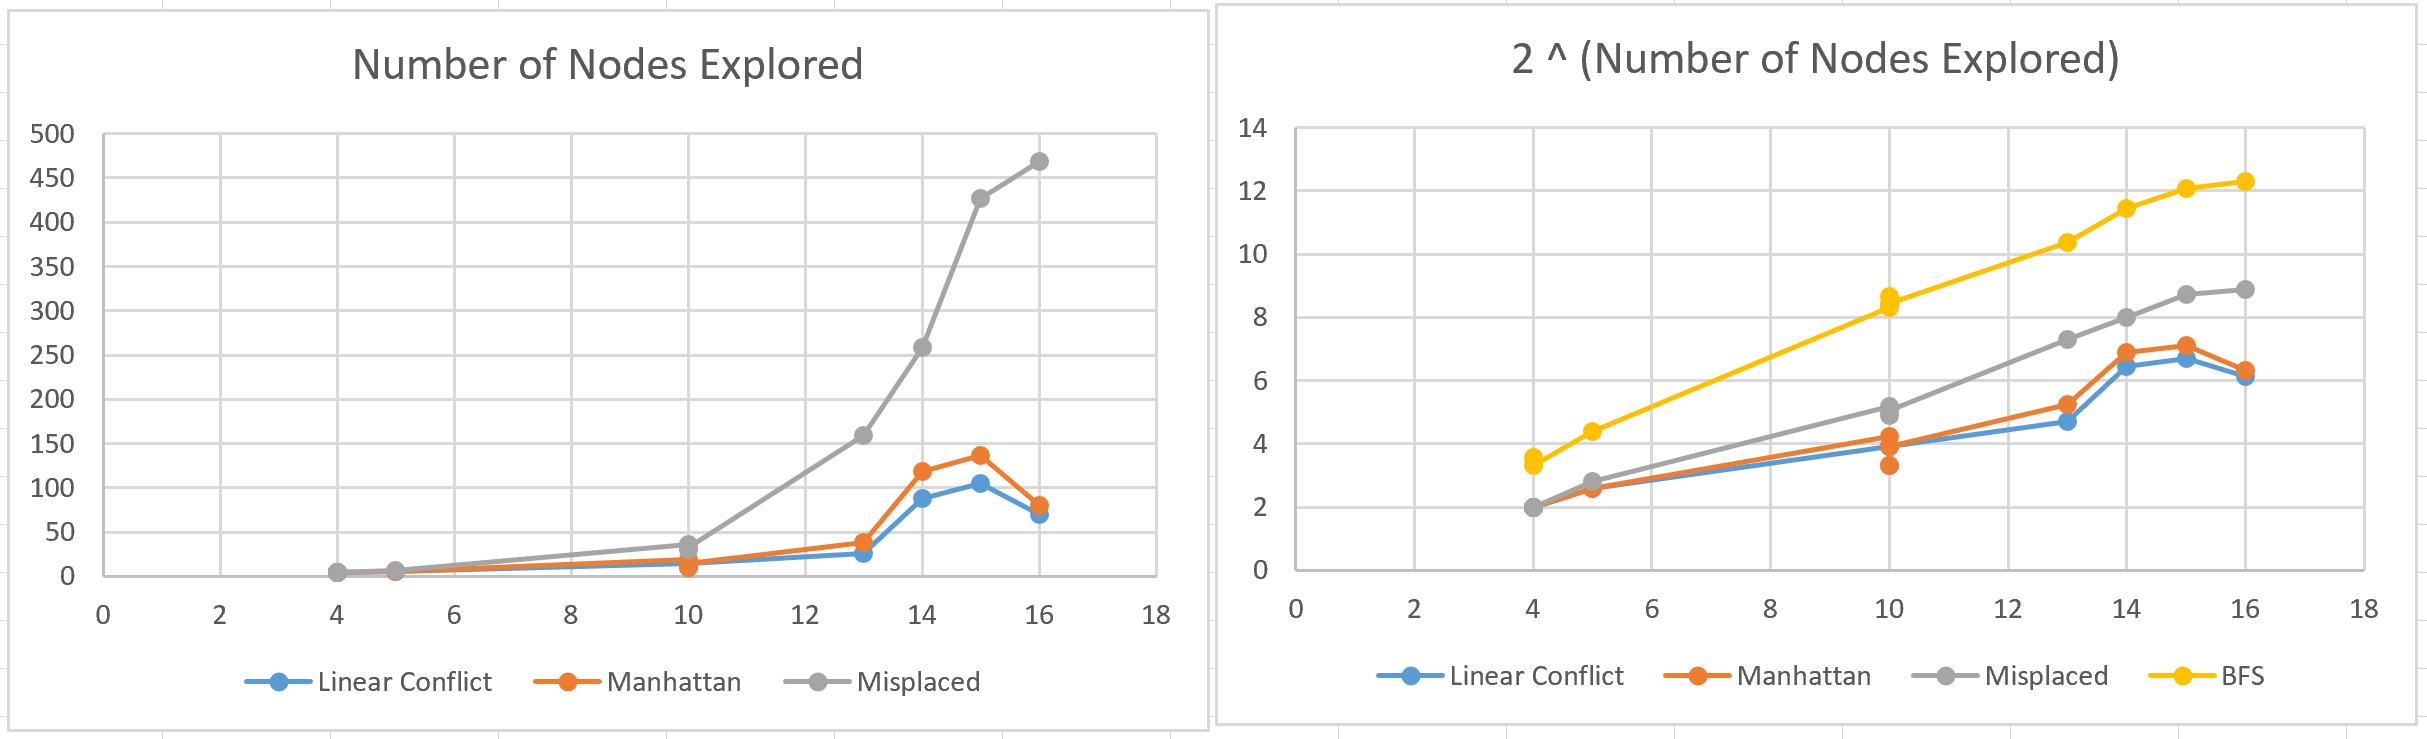
\includegraphics[width=\textwidth]{Results.PNG}
\caption{Number of nodes explored against length of optimal solution} \label{fig1}
\end{figure}

Overall, it is evident, that algorithms that can are proven theoretically faster on paper translate to real world speed up. 

\newpage

\section{To be deleted. Section for syntax reference}
\subsection{A Subsection Sample}
Please note that the first paragraph of a section or subsection is
not indented. The first paragraph that follows a table, figure,
equation etc. does not need an indent, either.

Subsequent paragraphs, however, are indented.

\subsubsection{Sample Heading (Third Level)} Only two levels of
headings should be numbered. Lower level headings remain unnumbered;
they are formatted as run-in headings.

\paragraph{Sample Heading (Fourth Level)}
The contribution should contain no more than four levels of
headings. Table~\ref{tab1} gives a summary of all heading levels.

\begin{table}
\caption{Table captions should be placed above the
tables.}\label{tab1}
\begin{tabular}{|l|l|l|}
\hline
Heading level &  Example & Font size and style\\
\hline
Title (centered) &  {\Large\bfseries Lecture Notes} & 14 point, bold\\
1st-level heading &  {\large\bfseries 1 Introduction} & 12 point, bold\\
2nd-level heading & {\bfseries 2.1 Printing Area} & 10 point, bold\\
3rd-level heading & {\bfseries Run-in Heading in Bold.} Text follows & 10 point, bold\\
4th-level heading & {\itshape Lowest Level Heading.} Text follows & 10 point, italic\\
\hline
\end{tabular}
\end{table}


\noindent Displayed equations are centered and set on a separate
line.
\begin{equation}
x + y = z
\end{equation}
Please try to avoid rasterized images for line-art diagrams and
schemas. Whenever possible, use vector graphics instead (see
Fig.~\ref{fig1}).

\begin{figure}
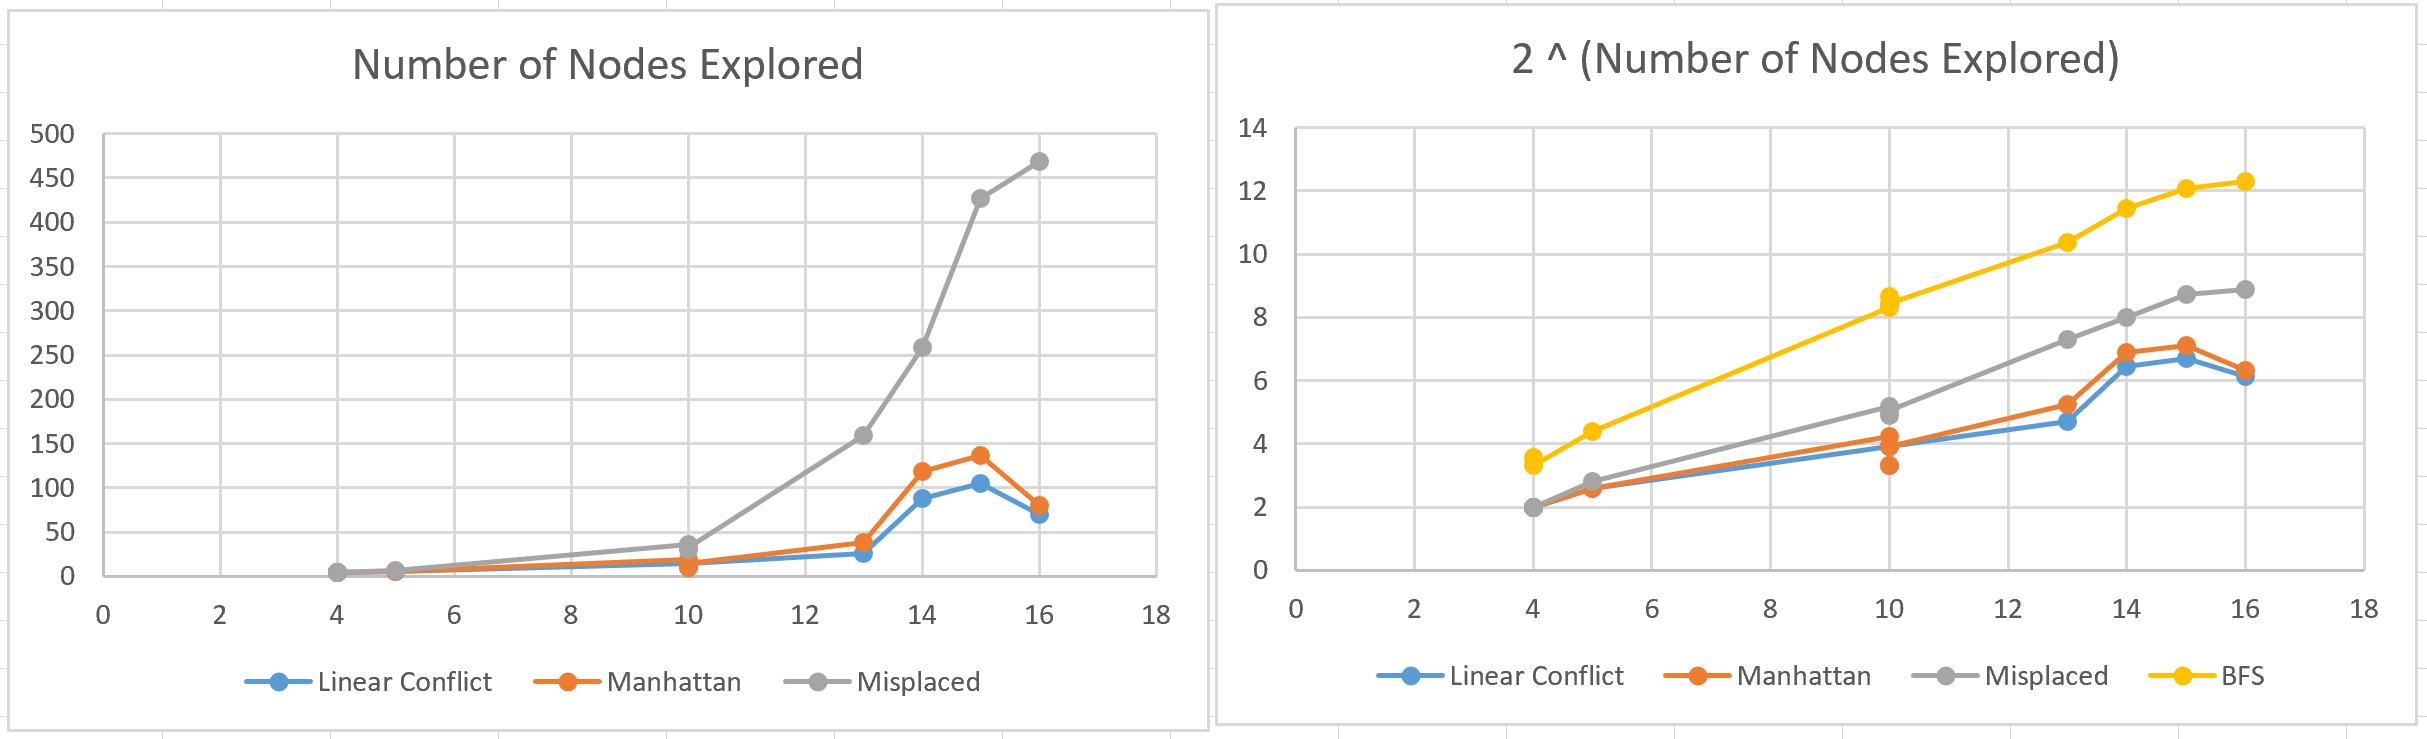
\includegraphics[width=\textwidth]{Results.PNG}
\caption{A figure caption is always placed below the illustration.
Please note that short captions are centered, while long ones are
justified by the macro package automatically.} \label{fig1}
\end{figure}

\begin{theorem}
This is a sample theorem. The run-in heading is set in bold, while
the following text appears in italics. Definitions, lemmas,
propositions, and corollaries are styled the same way.
\end{theorem}
%
% the environments 'definition', 'lemma', 'proposition', 'corollary',
% 'remark', and 'example' are defined in the LLNCS documentclass as well.
%
\begin{proof}
Proofs, examples, and remarks have the initial word in italics,
while the following text appears in normal font.
\end{proof}
For citations of references, we prefer the use of square brackets
and consecutive numbers. Citations using labels or the author/year
convention are also acceptable. The following bibliography provides
a sample reference list with entries for journal
articles~\cite{ref_article1}, an LNCS chapter~\cite{ref_lncs1}, a
book~\cite{ref_book1}, proceedings without editors~\cite{ref_proc1},
and a homepage~\cite{ref_url1}. Multiple citations are grouped
\cite{ref_article1,ref_lncs1,ref_book1},
\cite{ref_article1,ref_book1,ref_proc1,ref_url1}.
%
% ---- Bibliography ----
%
% BibTeX users should specify bibliography style 'splncs04'.
% References will then be sorted and formatted in the correct style.
%
% \bibliographystyle{splncs04}
% \bibliography{mybibliography}
%
\begin{thebibliography}{8}
\bibitem{ref_article1}
Author, F.: Article title. Journal \textbf{2}(5), 99--110 (2016)

\bibitem{ref_lncs1}
Author, F., Author, S.: Title of a proceedings paper. In: Editor,
F., Editor, S. (eds.) CONFERENCE 2016, LNCS, vol. 9999, pp. 1--13.
Springer, Heidelberg (2016). \doi{10.10007/1234567890}

\bibitem{ref_book1}
Author, F., Author, S., Author, T.: Book title. 2nd edn. Publisher,
Location (1999)

\bibitem{ref_proc1}
Author, A.-B.: Contribution title. In: 9th International Proceedings
on Proceedings, pp. 1--2. Publisher, Location (2010)

\bibitem{ref_url1}
LNCS Homepage, \url{http://www.springer.com/lncs}. Last accessed 4
Oct 2017
\end{thebibliography}
\end{document}
